%\documentclass[10pt,a4paper,addpoints]{exam}
\documentclass[10pt,a4paper,addpoints,answers]{exam}
\usepackage[T1]{fontenc}
\usepackage[utf8]{inputenc}
\usepackage[spanish]{babel}
\usepackage{multirow}
\usepackage{graphicx}
\usepackage{xcolor}
\usepackage{listings}
\usepackage{upquote}
\usepackage{xcolor}
\usepackage{listings}
\usepackage{amsmath}
\usepackage{tcolorbox}

\usepackage[scaled]{helvet} % Paquete para el tipo de letra
\renewcommand\familydefault{\sfdefault}

\usepackage{setspace} % Paquete para controlar el interlineado
\setstretch{1.1} 

% Para poder definir 3/4 Punto
\newcommand*\threequarters{%
  $\raise0.6ex\hbox{$\scriptstyle 3$}\kern -.2em/\kern -.2em
     \raise-0.5ex\hbox{$\scriptstyle 4$}$ Punto%
}


% Definición de colores
\definecolor{keywordcolor}{rgb}{0.1,0.1,0.8} % Azul para palabras clave
\definecolor{stringcolor}{rgb}{0.8,0.1,0.1}  % Rojo para cadenas
\definecolor{commentcolor}{rgb}{0.1,0.6,0.1} % Verde para comentarios

% Configuración de listings
\lstdefinestyle{mysqlstyle}{
  basicstyle=\ttfamily\footnotesize,          % Estilo básico
  keywordstyle=\color{keywordcolor}\bfseries, % Estilo para palabras clave
  commentstyle=\color{commentcolor}\itshape,  % Estilo para comentarios
  stringstyle=\color{stringcolor},            % Estilo para cadenas
  showstringspaces=false,                     % No mostrar espacios en cadenas
  tabsize=2,                                  % Tamaño de tabulación
  breaklines=true                             % Dividir líneas largas
}

\lstdefinelanguage{SQL}{
  morekeywords={RETURN, SELECT, INSERT, UPDATE, DELETE, FROM, WHERE, JOIN, INNER, LEFT, RIGHT, ON, GROUP, BY, ORDER, ASC, DESC, CREATE, TABLE, DROP, ALTER, DATABASE, USE, INDEX, INTO, VALUES, SET, IF, EXISTS, NOT, NULL, AND, HAVING, COUNT, DISTINCT, LIKE, IN, PROCEDURE, INTEGER, DECIMAL, TEXT, VARCHAR, BEGIN, DECLARE, INT, DEFAULT, CURSOR, FOR, CONTINUE, HANDLER, FOUND, OPEN, END, LOOP, ELSE, CLOSE, END, AFTER, BEFORE, EACH, ROW, NEW, OLD, THEN, SIGNAL, SQLSTATE, NATURAL, USER, IDENTIFIED, GRANT, TO, TRIGGER, PROCEDURE, FUNCTION, RETURNS, DETERMINISTIC, DELIMITER, OUT, PRIMARY, KEY, FOREIGN, REFERENCES, COMMIT, ELSEIF}, % Palabras clave SQL
  sensitive=false,
  morestring=[b]',                            % Cadenas con comillas simples
  morestring=[b]",                            % Cadenas con comillas dobles
  literate={ñ}{{\~n}}1                        % Permite el carácter "ñ"
}

% Usar el estilo
\lstset{style=mysqlstyle}

% Términos en castellano
\pointpoints{Punto}{Puntos}
\renewcommand{\solutiontitle}{\noindent\textbf{Solución propuesta:}\enspace\\}
\renewcommand{\questionlabel}{\textbf{Ejercicio \thequestion.}}

% Tabla para que el alumno introduzca sus datos
\def\studentdata{
    \begin{table}[t]
        \renewcommand{\arraystretch}{1.2}
        \small
        \centering
        \begin{tabular}{|l|p{4cm}|p{4cm}|p{2.5cm}|}
            \hline
            \multirow{3}{*}{
\includegraphics[width=2.5cm]{logos/etsisi}} & \multicolumn{3}{l|}{Apellidos:} \\ \cline{2-4} 
                                                                      & \multicolumn{3}{l|}{Nombre:}    \\ \cline{2-4} 
                                                                      & DNI:  & Num. mat.: & Grupo: \\ \hline
        \end{tabular}%
    \end{table}
}

% Estilo de la cabecera y pie de pagina
\pagestyle{headandfoot}
\firstpageheadrule
\runningheadrule
\header{Bases de Datos}{}{Convocatoria extraordinaria\\Curso 2025/2026}
\firstpagefootrule
\runningfootrule
\footer{}{}{Página\,\thepage\,de\,\numpages}

\begin{document}

\begin{center}\textbf{NORMATIVA DEL EXAMEN}\end{center}
\begin{itemize}
    \item Deberá escribir su nombre, con bolígrafo, en todas las hojas de las que consta el examen. Durante el examen, los profesores podrán solicitar acreditar la identidad de los participantes en el mismo. Deberá tener en todo momento su Documento Nacional de Identidad y/o Carné de la Universidad Politécnica de Madrid visible sobre la mesa.
    \item Los ejercicios deberán resolverse con bolígrafo, excepto el diagrama solicitado en el ejercicio 1, el cual podrá completarse opcionalmente a lápiz.
    \item Queda prohibido el uso de teléfonos móviles y cualquier otro dispositivo electrónico, los cuales deberán permanecer \textbf{apagados} durante toda la prueba. Se utilizarán sistemas de detección de radiofrecuencia para garantizar el cumplimiento de esta norma. En caso de detectarse un dispositivo encendido, se aplicará la \textit{Normativa sobre el uso de dispositivos detectores de radiofrecuencia y campo magnético en pruebas de evaluación}, aprobada por el Consejo de Gobierno de la Universidad Politécnica de Madrid el 26 de marzo de 2026.
    \item El examen tiene una duración máxima de \textbf{2 horas y 30 minutos}. No se permite abandonar el examen durante los primeros 20 minutos. Transcurrido este tiempo, no se permitirá la entrada al examen. 
    \item No está permitido el uso de libros ni apuntes durante el examen.
    \item Se prohíbe el uso de los operadores \texttt{MINUS}, \texttt{EXCEPT} e \texttt{INTERSECT} de SQL, así como de la claúsula \texttt{WITH}. Los apartados de los ejercicios en los que se utilicen serán calificados con 0 puntos.
    \item Durante el transcurso de la prueba \textbf{no se responderán dudas ni consultas relativas a la interpretación del texto del problema de modelado de datos}, dado que cualquier aclaración podría sugerir o revelar parte de la solución técnica. En caso de que el estudiante detecte alguna ambigüedad o falta de información explícita en el enunciado, deberá adoptar una decisión de diseño coherente. Es obligatorio que dichas decisiones queden reflejadas por escrito dentro de la solución entregada. La corrección valorará la coherencia de la solución en base a las suposiciones anotadas.
    \item Las calificaciones provisionales, junto con la fecha de revisión del examen, serán publicadas en el Moodle de la asignatura a los 15 días hábiles desde la fecha de realización del examen.
\end{itemize}

\vspace{1em}

\begin{center}\textbf{DECLARACIÓN DE COMPROMISO Y HONESTIDAD ACADÉMICA}\end{center}

Yo, D./D.a \rule{7cm}{0.4pt}, con DNI/NIE \rule{3cm}{0.4pt}, estudiante de la asignatura \textit{Bases de datos}, declaro bajo mi responsabilidad que:

\begin{enumerate}
    \item He leído y comprendo las instrucciones indicadas por el profesorado para la realización de este examen y me comprometo a cumplirlas en su totalidad.
    \item Me comprometo a realizar la prueba con honestidad académica, absteniéndome de cualquier forma de fraude, copia, suplantación de identidad o uso indebido de materiales no autorizados.
    \item Declaro que mantendré desconectados y fuera de uso todos los dispositivos electrónicos (teléfonos móviles, relojes inteligentes, auriculares, tabletas u otros similares), salvo aquellos estrictamente necesarios por motivos de salud, que deberán haber sido previamente comunicados y autorizados por el profesorado.
    \item Soy consciente de que el incumplimiento de cualquiera de estos compromisos podrá dar lugar a la aplicación de la normativa académica vigente en materia de evaluación y disciplina. 
\end{enumerate}

Y para que así conste, firmo la presente declaración antes del inicio del examen.

\vspace{3em}

\begin{center}En \textit{Madrid}, a 26 de Junio de 2026\end{center}

\newpage

\begin{questions}

\studentdata

\question[2] Modelado entidad relación

Realizar un modelo conceptual de datos mediante la técnica del modelo \textbf{Entidad Relación de Chen} teniendo en cuenta la siguiente descripción:

\begin{quotation}

La agencia InmoVallecas, líder en la gestión de activos residenciales en el distrito de Vallecas, se encuentra en un proceso de transformación digital. Con el fin de optimizar el seguimiento de su cartera de inmuebles y mejorar la eficiencia en sus procesos de venta, nos ha encomendado el diseño conceptual de su base de datos.

Cada uno de las viviendas que tienen pendientes de vender tiene asignado un código que lo identifica. Además de este código, se quiere conocer la dirección de la vivienda, la superficie, el número de habitaciones, el precio y la fecha de puesta en venta. Las viviendas están clasificados por zonas (porque a sus clientes, en ocasiones, sólo les interesan las viviendas de una zona determinada), y se quiere saber en qué zona está situado cada vivienda. Las zonas tienen un nombre de zona que es diferente para cada una de una misma población, pero que pueden coincidir en zonas de poblaciones diferentes. En ocasiones puede suceder que en algunas de las zonas no se tiene ningúna vivienda pendiente de vender. Sobre las poblaciones se quiere saber también el número de habitantes y tamaño en kilomentros cuadrados.

Se disponen de diferentes características de las viviendas, como por ejemplo tener ascensor, ser exterior, tener terraza, etc. Cada característica se identifica mediante un código y tiene una descripción. Para cada característica y cada vivienda se quiere saber si la vivienda satisface la característica o no. Además, quieren tener constancia del propietario principal de cada vivienda.

También se necesita disponer de información relativa a sus clientes actuales que buscan vivienda (si dos o más personas buscan vivienda conjuntamente, sólo se guarda información de una de ellas como cliente de la empresa). En particular, interesa saber las zonas donde busca vivienda cada cliente (sólo en caso de que tenga alguna zona de preferencia).

A cada uno de estos clientes le asignan un vendedor de la empresa para que se ocupe de atenderlo. A veces, estas asignaciones varían con el tiempo y se cambia al vendedor asignado a un determinado cliente. También es posible que a un cliente se le vuelva a asignar un vendedor que ya había tenido con anterioridad, y se quiere tener constancia de los períodos de todas estas asignaciones a lo largo del tiempo.

Los vendedores, clientes y propietarios se identifican por un código y se quiere registrar, de todos, su nombre, y número de teléfono. Además, se quiere disponer del número de Seguridad Social y el sueldo de los vendedores, y el NIF de los propietarios y clientes.

Finalmente, para ayudar a programar y consultar las visitas que los clientes hacen a las viviendas en venta, se quiere guardar información de todas las visitas correspondientes a los clientes y a las viviendas actuales de la empresa. De cada visita hay que saber el cliente que la hace, la vivienda que se va a ver, y el día y la hora concreta en que se inicia la visita. Hay que considerar que un mismo cliente puede visitar una misma vivienda varias veces para asegurarse de si le gusta o no, y también que para evitar conflictos no se programan nunca visitas de clientes diferentes a un misma vivienda y a la misma hora.

\end{quotation}

Se pide realizar un \textbf{modelo entidad-relación de Chen} justificando las  \textbf{cardinalidades mínimas} de al menos una relación (\textbf{ambos lados de la relación}) y un elemento de semántica no contemplada que se detecte.

\begin{solution}
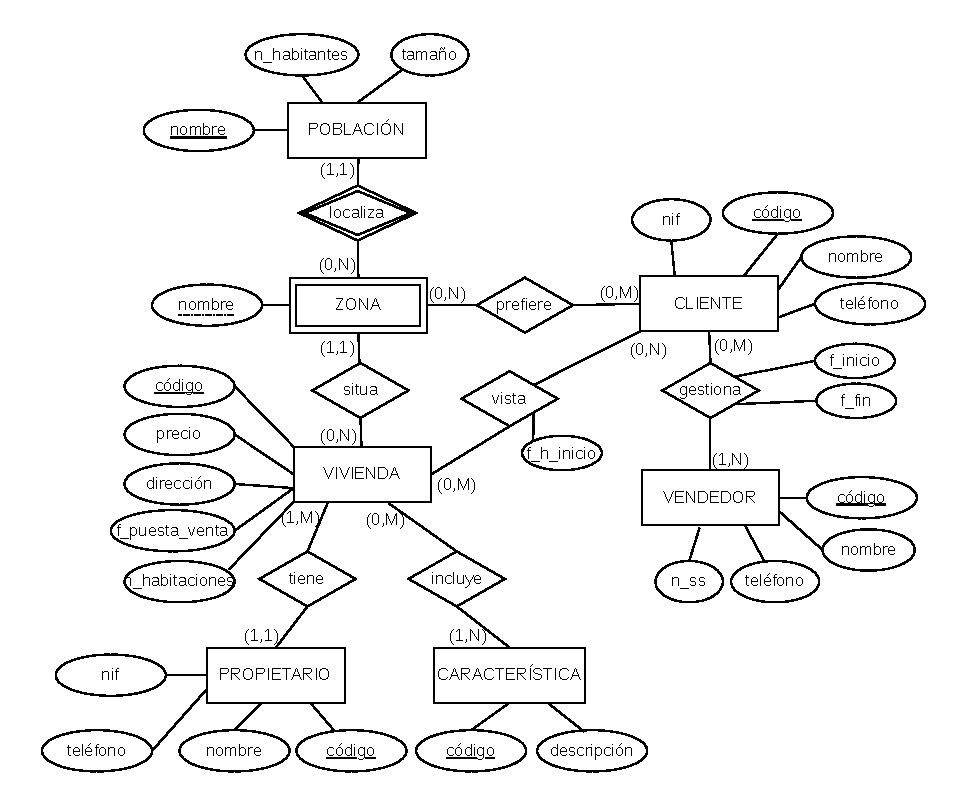
\includegraphics[width=\textwidth]{figs/bbdd-2025-2026-extraordinaria/InmoBBDD.pdf}

\textit{Cardinalidades mínimas}: La cardinalidad mínima de vivenda con respecto a zona es 1, ya que para todas las viviendas están ubicadas en una zona. Por otra parte, la cardinalidad mínima de zona con respecto a vivienda es 0, ya es posible que puedan existir zonas que no contengan viviendas en venta por parte de la inmobiliaria.

\textit{Semántica no contemplada}: No se puede registrar más de una visita para una misma vivienda el mismo día y hora. 

\end{solution}

% bloque de saltos de pagina para tener dos páginas en el MER
%\newpage
%~
%\newpage
%~
% fin del bloque de saltos de pagina


\newpage
\studentdata
\question[1\half] Dado el siguiente modelo relacional\footnote{Tenga en cuenta que las claves primarias aparecen \underline{subrayadas} mientras que las claves foráneas aparece en \textit{cursiva} junto con el superíndice \textsuperscript{FK} y comparten nombre con la clave primaria a la que referencian.} para la gestión de una red de estaciones de recarga para vehículos eléctricos:

\texttt{ESTACION (\underline{idEst}, ubicacion, estado)}

\texttt{PUNTO\_RECARGA (\underline{idPunto}, \textit{idEst}\textsuperscript{FK}, tipoConector, potenciaKW)}

\texttt{VEHICULO (\underline{matricula}, modelo, capacidadBateria, \textit{idUsuario}\textsuperscript{FK})}

\texttt{USUARIO (\underline{idUsuario}, nombre, NIF, email, tipoSuscripcion )}

\texttt{SESION\_CARGA (\underline{\textit{matricula}}\textsuperscript{FK}, \underline{\textit{idPunto}}\textsuperscript{FK}, \underline{fechaInicio}, fechaFin, energiaConsumidaKWh)}

Se pide dar respuesta a las siguientes cuestiones:

\begin{parts}

\part (\threequarters) Resolver mediante álgebra relacional: ``\textit{Obtener el nombre de los usuarios que poseen al menos un vehículo eléctrico con una capacidad de la batería superior a 70 y que han utilizado todos los puntos de recarga de la estación EST\_LUJO, pero que nunca han realizado una carga en la estación EST\_LOWCOST.}''.
\begin{solution}[20em]
\begin{align*}
    R_{usuarios\_potentes} &= \Pi_{idUsuario, nombre} \left( USUARIO \bowtie \sigma_{capacidadBateria > 70} (VEHICULO) \right ) \\
    R_{usuarios\_puntos} &= \Pi_{idUsuario, idPunto} \left( VEHICULO \bowtie SESION\_CARGA \right) \\
    R_{usuarios\_lujo} &= R_{usuarios\_puntos} \div \Pi_{idPunto}\left( \sigma_{idEst = EST\_LUJO} (PUNTO\_RECARGA) \right) \\
    R_{usuarios\_lowcost} &= \Pi_{idUsuario} ( R_{usuarios\_puntos} \bowtie PUNTO\_RECARGA \bowtie \\
    & \quad \bowtie \sigma_{idEst = EST\_LOWCOST} (ESTACION) ) \\
    R &= \Pi_{nombre}\left( R_{usuarios\_potentes} \bowtie ( R_{usuarios\_lujo} - R_{usuarios\_lowcost}) \right)
\end{align*}
\end{solution}

\part (\threequarters) Resolver mediante álgebra relacional: ``\textit{Obtener el idUsuario de aquellos usuarios que han cargado sus vehículos utilizando puntos de recarga de tipo 'CCS2' y que también han utilizado en alguna ocasión puntos de tipo 'Tesla'.}''.

\begin{solution}[10em]
\begin{align*}
    R1 &= \Pi_{idUsuario} ( VEHICULO \bowtie SESION\_CARGA \bowtie \\& \quad \bowtie \sigma_{tipoConector = CCS2} (PUNTO\_RECARGA) ) \\
    R2 &= \Pi_{idUsuario} ( VEHICULO \bowtie SESION\_CARGA \bowtie \\& \quad \bowtie \sigma_{tipoConector = Tesla} (PUNTO\_RECARGA) ) \\
    R &= R1 \cap R2
\end{align*}
\end{solution}

\end{parts}


\newpage
\studentdata
\question[3] En un contexto económico marcado por la volatilidad del precio de la energía, el excéntrico inversor Alan Máscara ha decidido lanzar una plataforma revolucionaria para la gestión de vehículos eléctricos. Para que la aplicación sea eficiente y escalable, es imperativo explotar la base de datos centralizada y extraer información crítica sobre el estado y uso de las estaciones de carga.

Por orden directa de Máscara, deberás resolver las siguientes consultas:

\begin{parts}


% creo que esta es sencilla pero hay que entenderla, he puesto una mas que en ordinaria porque poner una que valiera 1 punto me daba cosilla
\part (\threequarters) Resolver mediante SQL la siguiente consulta: ``\textit{Obtener el idEst y la ubicacion de aquellas estaciones cuya potencia media sea estrictamente superior a la potencia media de todas las estaciones de la red.}''
\begin{solution}[25em]
\begin{lstlisting}[language=SQL]
SELECT e.idEst, e.ubicacion
FROM ESTACION e JOIN PUNTO_RECARGA p ON e.idEst = p.idEst
GROUP BY e.idEst, e.ubicacion
HAVING AVG(p.potenciaKW) > (SELECT AVG(pm)
                            FROM (SELECT AVG(potenciaKW) AS pm
                                  FROM punto_recarga
                                  GROUP BY idEst) 
                            );
\end{lstlisting}
\end{solution}



\part (\threequarters) Resolver mediante SQL la siguiente consulta: ``\textit{Obtener los usuarios Premium que han utilizado, a través de cualquiera de sus vehículos, la totalidad de los puntos de recarga de más de 50kW en la estación 'EST\_CENTRO'.}''
\begin{solution}[24em]
\begin{lstlisting}[language=SQL]
SELECT u.nombre
FROM USUARIO u
WHERE u.tipoSuscripcion = 'Premium' 
        AND NOT EXISTS ( SELECT *
                         FROM PUNTO_RECARGA p
                         WHERE p.idEst = 'EST_CENTRO' AND p.potenciaKW > 50 
                                AND NOT EXISTS ( SELECT *
                                                 FROM SESION_CARGA s JOIN VEHICULO v ON s.matricula = v.matricula
                                                 WHERE s.idPunto = p.idPunto AND v.idUsuario = u.idUsuario  )
);
\end{lstlisting}
\end{solution}

%%AQUI METER SALTO DE PAGINA

\part (\threequarters) Resolver mediante SQL la siguiente consulta: ``\textit{Obtener el NIF y el nombre de los usuarios que poseen algún vehículo con \texttt{capacidadBateria} superior a 50 kWh. y que han realizado alguna carga con un conector tipo '`GBT', pero que \textbf{NUNCA} han utilizado un conector tipo `NACS'.}''
\begin{solution}[30em]
\begin{lstlisting}[language=SQL]
SELECT nombre, NIF 
FROM USUARIO 
WHERE idUsuario IN ( SELECT idUsuario 
                     FROM VEHICULO 
                     WHERE capacidadBateria > 50 )
AND idUsuario IN ( SELECT v.idUsuario 
                   FROM VEHICULO v 
                       JOIN SESION_CARGA s ON v.matricula = s.matricula
                       JOIN PUNTO_RECARGA p ON s.idPunto = p.idPunto
                   WHERE p.tipoConector = 'GBT' )
AND idUsuario NOT IN ( SELECT v.idUsuario 
                       FROM VEHICULO v 
                           JOIN SESION_CARGA s ON v.matricula = s.matricula
                           JOIN PUNTO_RECARGA p ON s.idPunto = p.idPunto
                       WHERE p.tipoConector = 'NACS' );
\end{lstlisting}
\end{solution}


\part (\threequarters) Resolver mediante SQL la siguiente consulta: ``\textit{Obtener la matrícula y el modelo de los vehículos que han realizado la mayor carga de la historia (máximo valor de \texttt{energiaConsumidaKWh}), de entre aquellos vehículos pertenecientes a propietarios tengan una suscripción que no sea de tipo Básica'.}''
\begin{solution}[25em]
\begin{lstlisting}[language=SQL]
SELECT v.matricula, v.modelo
FROM VEHICULO v JOIN SESION_CARGA s ON v.matricula = s.matricula
WHERE s.energiaConsumidaKWh = ( SELECT MAX(energiaConsumidaKWh) 
                                FROM SESION_CARGA)
AND v.idUsuario NOT IN ( SELECT idUsuario 
                         FROM USUARIO 
                         WHERE tipoSuscripcion = 'Basica' );
\end{lstlisting}
\end{solution}



\end{parts}


%%% PROCEDIMIENTOS, FUNCIONES Y TRIGGERS
\newpage
\studentdata
\question[2\half] Teniendo en cuenta el modelo relacional del ejercicio 2, complete las siguientes preguntas:

\begin{parts}

\part[1] Se busca limitar la energía consumida por los usuarios con suscripción ``\textit{basic}'' durante sus procesos de carga; para ello, codifica un \textbf{TRIGGER} que impida crear sesiones de carga cuya energía consumida sea superior al 75\% de la capacidad de la batería del vehículo, aplicando esta restricción exclusivamente a los usuarios con dicho nivel de suscripción.


\begin{solution}[37em]
\begin{lstlisting}[language=SQL]
DELIMITER $$
CREATE TRIGGER limitar_carga
BEFORE INSERT ON sesion_carga
FOR EACH ROW
BEGIN
    DECLARE sus VARCHAR(10);
    DECLARE cap DECIMAL(10,2);

    SELECT tipoSuscripcion INTO sus
    FROM usuario 
        INNER JOIN vehiculo ON vehiculo.idUsuario = usuario.idUsuario
    WHERE matricula = NEW.matricula;

    IF sus = "basic" THEN
        SELECT capacidadBateria INTO cap
        FROM vehiculo
        WHERE matricula = NEW.matricula;

        IF NEW.energiaConsumidaKWh > 0.75 * cap THEN 
            SIGNAL SQLSTATE "02000"
            SET MESSAGE_TEXT = "La energia consumida no puede exceder el 75% de la capacidad de carga del vehiculo en usuarios 'basic'";
        END IF;
    END IF;
END$$
DELIMITER ;

\end{lstlisting}
\end{solution}

\part[1\half] Se desean instalar nuevos puntos de recarga y, para elegir las ubicaciones más adecuadas, se realizará un análisis de las sesiones de carga registradas en los últimos años. Con el fin de agilizar la analítica de datos, se empleará un software de visualización que requiere que la información sea procesada y entregada siguiendo estrictamente el siguiente formato:

\vspace{1em}
\begin{verbatim}
ubicacion 1|potencia total en ub. 1|energia consumida en ub. 1
ubicacion 2|potencia total en ub. 2|energia consumida en ub. 2
...
ubicacion n|potencia total en ub. n|energia consumida en ub. n
\end{verbatim}
\vspace{1em}

En este formato, \texttt{ubicacion i} representa el nombre de la ubicación en la base de datos, mientras que la \texttt{potencia total en ub. i} se define como la suma de las potencias de todos los puntos de recarga de dicha ubicación. Por su parte, la \texttt{energia consumida en ub. i} corresponde al sumatorio de la energía total consumida por las sesiones de carga iniciadas en ese lugar en el periodo analizado. 

Se solicita realizar un \textbf{PROCEDIMIENTO ALMACENADO} que devuelva, mediante un parámetro de salida de tipo \texttt{TEXT}, los datos formateados según el año pasado como parámetro. Es obligatorio utilizar la función \texttt{CONCAT} para concatenar cadenas de texto y la función \texttt{YEAR} para extraer el año de la \textit{fechaInicio}.

Como ejemplo, considera un escenario donde se analizan la sesiones de carga del año 2025. Ante una llamada como \texttt{CALL obtener\_estadisticas\_recargas(2025, @data);}, si en la ubicación de \texttt{madrid-retiro} existen dos puntos de carga de $150$ kW, en \texttt{sevilla-centro} hay un punto de carga de $44$ kW y en \texttt{bilbao-norte} hay tres puntos de recarga de $50$ kW, la variable de usuario \texttt{@data} debería contener una cadena de texto similar a la siguiente:

\vspace{1em}
\begin{verbatim}
madrid-retiro|300|145200
sevilla-centro|44|38600
bilbao-norte|150|52100
\end{verbatim}
\vspace{1em}

\begin{solution}[45em]
\begin{lstlisting}[language=SQL]
DELIMITER $$
CREATE PROCEDURE obtener_estadisticas_recargas (IN y INTEGER, OUT data TEXT)
BEGIN  
    DECLARE done INT DEFAULT FALSE;
    DECLARE ub VARCHAR(200);
    DECLARE sumPotencia DECIMAL(10,2); 
    DECLARE sumEnergia DECIMAL(10,2);    

    DECLARE cur CURSOR FOR 
        SELECT ubicacion, SUM(potenciaKW), SUM(energiaConsumida)
        FROM estacion
            INNER JOIN punto_recarga ON punto_recarga.idEst = estacion.idEst
            INNER JOIN sesion_carga ON sesion_carga.idPunto = punto_recarga.idPunto
        WHERE YEAR(fechaInicio) = y
        GROUP BY ubicacion;
                             
    DECLARE CONTINUE HANDLER FOR NOT FOUND SET done = TRUE;

    SET data = '';
    
    OPEN cur;
    read_loop: LOOP       
        FETCH cur INTO ub, sumPotencia, sumEnergia;

        IF done THEN
            LEAVE read_loop;
        END IF;
        
        SET data = CONCAT(data, ub, '|', sumPotencia, '|', sumEnergia, '\n');

    END LOOP;
    CLOSE cur;
END$$
DELIMITER ;

\end{lstlisting}
\end{solution}

\end{parts}

\newpage
\studentdata

\question[1] Tomando como referencia el uso habitual que se hace de la información de la base de datos del ejercicio 2, representa en JSON embebido la estructura de una estación de recarga con sus puntos y sesiones, identificando los vehículos mediante su matrícula y permitiendo obtener, a partir de ellos, los datos del usuario correspondiente. Justifica la respuesta.

\vspace{1em}

\begin{tabular}{ccc}
\hline
\textbf{idEst} & \textbf{ubicacion} & \textbf{estado} \\ \hline
1              & madrid-retiro      & Activa          \\ \hline
\end{tabular}

\vspace{1em}

\begin{tabular}{cccc}
\hline
\textbf{idPunto} & \textbf{idEst} & \textbf{tipoConector} & \textbf{potenciaKW} \\ \hline
101	             & 1              & CCS2                  & 150                 \\ \hline
102	             & 1              & Type 2                & 150                 \\ \hline
\end{tabular}

\vspace{1em}

\begin{tabular}{ccccc}
\hline
\textbf{idUsuario} & \textbf{nombre} & \textbf{NIF} & \textbf{email} & \textbf{tipoSuscripcion} \\ \hline
1                  & Ana López       & 12345678A    & ana@email.com  & Premium                  \\ \hline
\end{tabular}

\vspace{1em}

\begin{tabular}{cccc}
\hline
\textbf{matricula} & \textbf{modelo} & \textbf{capacidadBateria} & \textbf{idUsuario} \\ \hline
1111ABC            & Tesla Model 3   & 75.0                      & 1                  \\ \hline
5555EFG            & Kia EV6         & 77.4                      & 1                  \\ \hline
\end{tabular}

\vspace{1em}

\begin{tabular}{ccccc}
\hline
\textbf{matricula} & \textbf{idPunto} & \textbf{fechaInicio} & \textbf{fechaFin}   & \textbf{energiaConsumidaKWh} \\ \hline
1111ABC            & 101              & 2025-01-10 08:00:00  & 2025-01-10 09:15:00 & 18.5                         \\ \hline
5555EFG            & 101              & 2025-07-07 08:15:00  & 2025-07-07 09:30:00 & 25.0                         \\ \hline
1111ABC            & 102              & 2025-02-12 10:00:00  & 2025-02-12 11:10:00 & 16.0                         \\ \hline
\end{tabular}

\vspace{1em}

\begin{solution}[12em]
La estación, sus puntos y las sesiones se embeben porque forman la parte operativa que normalmente se consulta de manera conjunta. 
En cambio, los vehículos se dejan como colección separada y se identifican en las sesiones mediante \texttt{matricula}, lo que evita repetir datos; a partir de esa matrícula puede recuperarse el vehículo y, por su \texttt{idUsuario}, el usuario asociado. Con los datos dados el JSON quedará

\begin{verbatim}
{
  "estacion": {
    "idEst": 1,
    "ubicacion": "madrid-retiro",
    "estado": "Activa",
    "puntosRecarga": [
      {
        "idPunto": 101,
        "tipoConector": "CCS2",
        "potenciaKW": 150,
        "sesionesCarga": [
          {
            "fechaInicio": "2025-01-10 08:00:00",
            "fechaFin": "2025-01-10 09:15:00",
            "energiaConsumidaKWh": 18.5,
            "matricula": "1111ABC"
          },
          {
            "fechaInicio": "2025-07-07 08:15:00",
            "fechaFin": "2025-07-07 09:30:00",
            "energiaConsumidaKWh": 25.0,
            "matricula": "5555EFG"
          }
        ]
      },
      {
        "idPunto": 102,
        "tipoConector": "Type 2",
        "potenciaKW": 150,
        "sesionesCarga": [
          {
            "fechaInicio": "2025-02-12 10:00:00",
            "fechaFin": "2025-02-12 11:10:00",
            "energiaConsumidaKWh": 16.0,
            "matricula": "1111ABC"
          }
        ]
      }
    ]
  },
  "vehiculos": [
    {
      "matricula": "1111ABC",
      "modelo": "Tesla Model 3",
      "capacidadBateria": 75.0,
      "idUsuario": 1
    },
    {
      "matricula": "5555EFG",
      "modelo": "Kia EV6",
      "capacidadBateria": 77.4,
      "idUsuario": 1
    }
  ],
  "usuarios": [
    {
      "idUsuario": 1,
      "nombre": "Ana López",
      "NIF": "12345678A",
      "email": "ana@email.com",
      "tipoSuscripcion": "Premium"
    }
  ]
}
\end{verbatim}
\end{solution}

\end{questions}
\end{document}
